\documentclass
  [11pt,
   paper=a4,
   cleardouble=plain,
   chapterprefix=true,
   parskip=half,
   draft=true]
  {scrbook}

\usepackage[dutch]{babel}
\usepackage[T1]{fontenc}
\usepackage[utf8]{inputenc}

\usepackage{amsmath}
\usepackage{amssymb}

\usepackage{pxfonts}

\usepackage{tikz}
\usetikzlibrary{calc}
\tikzstyle{every picture}=[thick]

\usepackage{listings}
\lstdefinelanguage{proto}
  {keywords={var, obj, clones, fun, returns, is,
             print, skip,
             if, then, else, while, do},
   emph={true, false, this, proto},
   %literate={==}{{$=$}}1 {/=}{{$\neq$}}1 {<=}{{$\leq$}}1 {>=}{{$\geq$}}1
   %         {+}{{$+$}}1 {-}{{$-$}}1 {*}{{$\times$}}1 {/}{{$/$}}
   %         {&}{{$\wedge$}}1 {|}{{$\vee$}}1 {~}{{$\lnot$}}1,
   comment=[l]{\#}}
\lstdefinelanguage{io}
  {keywords={clone, method, block, call, return,
             print, println,
             if, then, else, elsif,
             loop, repeat, while, for, break, continue},
   emph={true, false, nil, self, super},
   comment=[l]{\#}}
\lstdefinelanguage{class}[]{proto}
  {morekeywords={extends},
   deletekeywords={clones},
   moreemph={super},
   deleteemph={proto}}
\lstnewenvironment{program}{}{}
\lstMakeShortInline @
\lstset
  {language=proto,
   basicstyle=\small\ttfamily,
   emphstyle=\scshape,
   numbers=left,
   numberstyle=\small,
   numbersep=1em,
   mathescape=true,
   extendedchars=true}

\usepackage[nounderscore]{syntax}
\setlength{\grammarindent}{8em}
\renewcommand{\syntleft}{\normalfont\itshape}
\renewcommand{\syntright}{}

\newcommand\newkeyword[2]
  {\newcommand{#1}
     {\text{\small\ttfamily\bfseries #2}}}
\newcommand\newconstant[2]
  {\newcommand{#1}
     {\text{\small\ttfamily\scshape #2}}}

\newcommand{\syn}[1]
  {\ensuremath{\mathit{#1}}}

\newcommand{\COMP}{;\;}
\newkeyword{\VAR}{var\;}
\newkeyword{\OBJ}{obj\;}
\newkeyword{\CLONES}{\;clones\;}
\newkeyword{\FUN}{fun\;}
\newkeyword{\RETURNS}{\;returns\;}
\newkeyword{\IS}{\;is\;}
\newkeyword{\PRINT}{print\;}
\newkeyword{\SKIP}{skip}
\newkeyword{\IF}{if\;}
\newkeyword{\THEN}{\;then\;}
\newkeyword{\ELSE}{\;else\;}
\newkeyword{\WHILE}{while\;}
\newkeyword{\DO}{\;do\;}
\newkeyword{\END}{\;end}

\newconstant{\TRUE}{true}
\newconstant{\FALSE}{false}
\newconstant{\SELF}{self}
\newconstant{\PROTO}{proto}

\newcommand{\<}
  {\ensuremath{\langle}}
\renewcommand{\>}
  {\ensuremath{\rangle}}

\frenchspacing% Cruciaal!
\raggedbottom% Handig

\begin{document}

\title{Een natuurlijke semantiek voor prototype gebaseerde talen}
\author{Kelley van Evert \& Tim Steenvoorden}
\maketitle

\frontmatter

\tableofcontents

\mainmatter

\chapter{Inleiding}

\begin{itemize}
	\item Motivatie
	\item JavaScript
	\item Lexical scope -- vrije/gebeonden variabelen
	\item Objecten en prototype overerving
\end{itemize}

\chapter{Notatie en terminologie}

\section{Beschouwing semantisch model}

We definieren in dit werkstuk een natuurlijke semantiek, d.w.z.~een ?-ste orde logica, met axioma's en deductieregels, en een bijbehorende structuur waarin deze zich afspeelt.

Deze structuur, die we ook wel het \emph{semantisch model} zullen noemen, heeft onderstaand opgesomde elementen. Deze worden verderop precies gedefinieerd, onderstaande opsomming geeft slechts een algemeen beeld.

\begin{description}
	\item[$\mathbb{M}$]\hfill\\ De verzameling mogelijke \emph{geheugens}, welke ook wel als \emph{eindtoestanden} worden geinterpreteerd.
	\item[$(\mathit{Stm} \times \mathbb{M} \times \mathbb{L} \times \mathbb{L})$]\hfill\\ De verzameling \emph{toestanden}, ook wel \emph{configuraties}.
	\item[$(\longrightarrow)$]\hfill\\ Een tweeplaatsig predikaat welke als eerste argument een element uit de verzameling van toestanden neemt, en als tweede argument een element uit de verzameling van eindtoestanden $(\mathbb{M}\dots)$. De uitspraak $(S, m, \sigma, \tau) \longrightarrow m'$ moet worden geinterpreteerd worden als:
	\begin{quote} ``Het programma $S$, met geheugen $m$, in scope $\sigma$ en met als $\mathbf{this}$ object $\tau$, resulteert in eindtoestand $m'$, mits $S$ \emph{correct} is''. \end{quote}
\end{description}

\section{Notationele conventies}

Terwille van elegantie houden we een aantal gebruikelijke notationele conventies aan:

\begin{enumerate}
	\item Voor elke twee willekeurige tweestemmige predikaten $\mathsf{S}$ en $\mathsf{T}$ (mogelijk ook $=$), en drie willekeurige elementen $a$, $b$ en $c$, definieren we de afkorting: $$a \operatorname{\mathsf{S}} b \operatorname{\mathsf{T}} c \buildrel{\mathrm{def}}\over{=} a \operatorname{\mathsf{S}} b \land b \operatorname{\mathsf{T}} c$$ in het geval dat deze bewering correct getypeerd is.
	\item Op eenzelfde manier definieren we ook de volgende afkorting: $$ \{a \in A \mid \phi \} \buildrel{\mathrm{def}}\over{=} \{a \mid a \in A \mid \phi\}$$
\end{enumerate}

[...]

\chapter{Syntax}

\section{Voorbeeldprogramma's}

[Ter motivatie en duidelijkheid]

\section{Grammatica}

[...en vervolgens helemaal formeel -- even uitleggen van BNF etc..]

\chapter{Semantisch model}

[Stukje bij beetje het semantisch model opbouwen, terwijl we steeds redeneren waarom we dat zo doen..]

\section{Scopes en lexical scope}

[Hierarchieen, outer scopes, bindingen, ``waarden'' kort noemen maar uitstellen tot ``Waarden: referenties en primitieven'']

\section{Objecten en prototype overerving}

[Graaf, bindingen, prototypen]

\section{Waarden: referenties en primitieven}

[Ze worden op dezelfde manier behandeld: objecten by-reference, dus de references zelf by-value, net als primitieven -- vandaar dat ze in dezelfde verzameling waarden zitten.]

\chapter{Case study: [benaming?]}

\chapter{[...]}

%\chapter{Syntaxis}

\section{Grammatica}

\begin{grammar}
<Statement>  ::= <Statement> ";" <Statement>
            \alt @skip@
            \alt @if@ <Test> <Statement> @else@ <Statement>
            \alt @while@ <Test> <Statement>
            \alt @print@ <Expression>
            \alt @var@ <Slots> 
            \alt <Slot> "=" <Expression>
            \alt @fun@ <Slot> "(" <Identifiers>? ")" [@returns@ <Slot>] <Statement>
            \alt [<Slot> "="] <Slot> "(" <Expressions>? ")"
            \alt @obj@ <Slot> [@clones@ <Slot>]

<Slot>       ::= <Identifier> | <Identifier> "." <Slot>

<Slots>       ::= <Slot> | <Slot> "," <Slots>

<Identifier> ::= ( "a" | \dots | "z" | "A" | \dots | "Z" | "_" )+

<Identifiers> ::= <Identifier> | <Identifier> "," <Identifiers>

<Expression> ::= <Number>
            \alt <Slot>
            \alt <Expression> <Operator> <Expression>

<Expressions> ::= <Expression> | <Expression> "," <Expressions>

<Operator>   ::= "+" | "-" | "*" | "/" | "\%"

<Number>     ::= ( "0" | \dots | "9" )+

<Test>       ::= <Boolean>
            \alt <Test> "\&" <Test>
            \alt <Test> "|"  <Test>
            \alt "~" <Test>
            \alt <Expression> <Relation> <Expression>

<Relation>   ::= "==" | "/=" | "<" | "<=" | ">" | ">="

<Boolean>    ::= @true@ | @false@
\end{grammar}

\section{Een programma over deuren}

\begin{program}
obj Door clones Object       // Maak een nieuwe deur

fun Door.open()              // Een functie om de deur te openen
    print 42

obj LockedDoor clones Door   // Maak een nieuwe gesloten deur...
var LockedDoor.isLocked
LockedDoor.isLocked = 1      // ...die dicht is

fun LockedDoor.unlock(code)
    if code == this.code     // Als de code correct is...
        isLocked = 0         // ...openen we de deur

fun LockedDoor.open()        // Herdefinieer om isLocked te gebruiken
    if isLocked == 1
        print 0
    else
        proto.open()         // Expliciete aanroep naar prototype

obj Safe clones LockedDoor   // Maak een kluis...
var Safe.code
Safe.code = 1234             // ...en ken een code toe

Safe.unlock(4321)
Safe.open()                  // Geeft 0, de deur is gesloten
Safe.unlock(1234)
Safe.open()                  // Geeft 42, we de juiste code hadden
\end{program}

\section{Een programma over personen}

\begin{program}
obj Person clones Object

var Person.total
Person.total = 0

fun Person.initialize()      // Wordt aangeroepen bij iedere kloon
    Person.total = Person.total + 1

obj Me clones Person
var Me.age
Me.age = 37

obj You clones Person
var You.age
You.age = 42

print Person.total           // Geeft 2
\end{program}

\section{Een programma over scope}

\begin{program}
var x
x = 1
fun g()
    print x
    x = 2
fun f()
    var x
    x = 3
    g()
f()
print x
\end{program}

\section{Een programma over counters}

\begin{minipage}{0.5\textwidth}
\begin{program}
fun counter(n) returns next

    fun next() returns n
        n = n + 1

var c
c = counter(5)

var d
d = counter(42)

var i, j
i = c() // i = 6
j = d() // j = 43
\end{program}
\end{minipage}
\begin{minipage}{0.5\textwidth}
\begin{program}
obj Counter clones Object
var Counter.n
fun Counter.next()
    n = n + 1

obj c clones Counter
c.n = 5

obj d clones Counter
d.n = 42


c.next() // c.n = 6
d.next() // d.n = 43
\end{program}
\end{minipage}

% vim: spell spl=nl

%\chapter{Vergelijking met IO}

\section{Grammatica}

\begin{grammar}
<Statement>  ::= <Statement> ";" <Statement>
            \alt "nil"
            \alt "if" "(" <Test> "," <Statement> "," <Statement> ")"
            \alt "while" "(" <Test> "," <Statement> ")"
            \alt <Expression> "println"
            \alt <Slot> ":=" <Expression>
            \alt <Slot>  "=" <Expression>
            \alt <Slot> ":=" "method" "(" \{ <Identifier> "," \} <Statement> ")"
            \alt <Slot> ":=" <Slot> "(" [ <Expression> \{ "," <Expression> \} ] ")"
            \alt <Slot> ":=" <Slot> "clone"

<Slot>       ::= <Identifier> \{ "\ " <Identifier> \}

<Identifier> ::= ( "a" | \dots | "z" | "A" | \dots | "Z" | "_" )+

<Expression> ::= <Number>
            \alt <Slot>
            \alt <Expression> <Operator> <Expression>

<Operator>   ::= "+" | "-" | "*" | "/"

<Number>     ::= ( "0" | \dots | "9" )+

<Test>       ::= <Boolean>
            \alt <Test> "and" "(" <Test> ")"
            \alt <Test> "or" "(" <Test> ")"
            \alt "not" "(" <Test> ")"
            \alt <Expression> <Relation> <Expression>

<Relation>   ::= "==" | "!=" | "<" | "<=" | ">" | ">="

<Boolean>    ::= "true" | "false"
\end{grammar}

\newpage
\section{Doors}

\begin{minipage}{0.5\textwidth}
\begin{program}
obj Door clones Object

fun Door.open() is
    print 42

obj LockedDoor clones Door
var LockedDoor.isLocked
LockedDoor.isLocked = 1

fun LockedDoor.unlock(code) is
    if code == this.code then
        isLocked = 0

fun LockedDoor.open() is
    if isLocked == 1 then
        print 0
    else
        proto.open()

obj Safe clones LockedDoor
var Safe.code
Safe.code = 1234

Safe.unlock(4321)
Safe.open()
Safe.unlock(1234)
Safe.open()
\end{program}
\end{minipage}
\begin{minipage}{0.5\textwidth}
\lstinputlisting[language=io]{doors.io}
\end{minipage}

\newpage
\section{Persons}

\begin{minipage}{0.5\textwidth}
\begin{program}
obj Person clones Object

var Person.total
Person.total = 0

fun Person.initialize() is
    Person.total = Person.total + 1

obj Me clones Person
var Me.age
Me.age = 37

obj You clones Person
var You.age
You.age = 42

print Person.total
\end{program}
\end{minipage}
\begin{minipage}{0.5\textwidth}
\lstinputlisting[language=io]{persons.io}
\end{minipage}

\section{Scope}

\begin{minipage}{0.5\textwidth}
\begin{program}
var x
x = 1
fun g() is
    print x
    x = 2
fun f() is
    var x # Weghalen geeft dynamic
    x = 3
    g()
f()
print x
\end{program}
\end{minipage}
\begin{minipage}{0.5\textwidth}
\lstinputlisting[language=io]{scope.io}
\end{minipage}

\newpage
\section{Counters}

\begin{minipage}{0.5\textwidth}
\begin{program}
fun counter(n) returns next is
    fun next() returns n is
        n = n + 1

var c
c = counter(5)

var d
d = counter(42)

var i, j
i = c()
j = d()
\end{program}
\end{minipage}
\begin{minipage}{0.5\textwidth}
\begin{lstlisting}[language=io]
counter := block(n,
    block(
        n = n + 1))


c := counter call(5)


d := counter call(42)


i := c call
j := d call
\end{lstlisting}
\end{minipage}

\begin{minipage}{0.5\textwidth}
\begin{program}
obj Counter clones Object
var Counter.n
fun Counter.next() is
    n = n + 1

obj c clones Counter
c.n = 5

obj d clones Counter
d.n = 42


c.next()
d.next()
\end{program}
\end{minipage}
\begin{minipage}{0.5\textwidth}
\begin{lstlisting}[language=io]
Counter := Object clone

Counter next := method(
    n = n + 1)

c := Counter clone

c n := 5

d := Counter clone

d n := 42

c next
d next
\end{lstlisting}
\end{minipage}

% vim: ft=context

%\chapter{Troep}

\section{Regels}

\subsection{While}

@$\<$while not (x = 1) do y = y * x; x = x - 1$, s_{3,2}\> \to s_{6,1}$@

$\<\WHILE x \neq 1 \DO y = y \times x;~ x = x - 1, s_{3,2}\> \to s_{6,1}$

$\<\mathtt{while}(x \neq 1, y = y \times x;~ x = x - 1), s_{3,2}\> \to s_{6,1}$

$\<\FUN counter(n) \RETURNS next \IS (\FUN next() \RETURNS n \IS n = n + 1), s\>$

$\<\FUN counter(n) \RETURNS next \IS \FUN next() \RETURNS n \IS n = n + 1 \END \END, s\>$

$\<counter := \mathtt{block}(n, \mathtt{block}(n = n + 1)), s\>$

$\<\VAR x\COMP x=1\COMP
   \FUN g() \IS (\PRINT x\COMP x=2)\COMP
   \FUN f() \IS (\VAR x\COMP x=3\COMP g())\COMP
   f()\COMP
   \PRINT x,
s\> \to s'$


$\<\VAR x\COMP x=1\COMP
   \FUN g() \IS \PRINT x\COMP x=2 \END\COMP
   \FUN f() \IS \VAR x\COMP x=3\COMP g() \END\COMP
   f()\COMP
   \PRINT x,
s\> \to s'$

$\<x:=1;~
   g:=\mathtt{method}(x \mathtt{~print};~ x=2);~
   f:=\mathtt{method}(x:=3;~ g());~
   f();~
   x \mathtt{~print}, 
s\> \to s'$

$\<x:=1;
   g:=\mathtt{block}(x \mathtt{~println}; x=2);
   f:=\mathtt{block}(x:=3; g \mathtt{~call});
   f \mathtt{~call};
   x \mathtt{~println}, 
s\> \to s'$

\subsection{Fun}

\<@fun $f$($y$) {$x$ = $y$}@, $s$, $\epsilon$\> $\to (s',\epsilon)$

@$\<$fun $f$($y$) {$x$ = $y$}$, s, \epsilon\> \to (s',\epsilon)$@

\<@fun f(y) {x = y}@, $s$, $\epsilon$\> $\to (s',\epsilon)$

$\<\FUN f(y) \IS x = y, s, \epsilon\> \to (s', \epsilon)$

---

$\< \mathbf{fun}\;f(y)\;\;\{x=y\}, s, \epsilon \> \to s'$

$\<\texttt{\FUN\ f(y) \{x = y\}}, s, \epsilon\> \to s'$

$\<\syn{fun f(y) {x = y}}, s, \epsilon\> \to s'$

%$\<@fun@ f@(@y@)@ @{@ x @=@ y@}@, s, \epsilon\> \to s'$

$\<\mathtt{fun} f(y) \{x = y\}, s, \epsilon\> \to s'$

\<@fun@ $f$@(@$y$@)@ @{@ $x$@=@$y$ @}@, $s$, $\epsilon$\> $\to s'$

--- ---

\subsection{If}

\<@if $T$ $S_1$ else $S_2$@, $s$, $\epsilon$\> $\to (s',\epsilon)$

@$\<$if $T$ $S_1$ else $S_2, s, \epsilon\> \to (s',\epsilon)$@

\<@if b T else F@, $s$, $\epsilon$\> $\to (s',\epsilon)$

---

$\<\syn{if T S1 else S2}, s\> \to s'$

$\<\IF\; T\; S_1\; \ELSE\; S_2, s\> \to s'$

%$\langle @if@ T S_1 @else@ S_2, s \rangle \to s'$

$\langle$@if T S1 else S2@$\rangle$

@$\langle$ if $T$ $S_1$ else $S_2$ $\rangle$@

\<@if@ $T$ $S_1$ @else@ $S_2$, $s$\> $\to s'$

%$\< @if@\; T\; S_1\; @else@\; S_2, s \> \to s'$

$\< \IF T S_1 \ELSE S_2 \> \to s'$

%\tuple{@if@ $T$ $S_1$ @else@ $S_2$}$\to s'$

\section{Bomen}

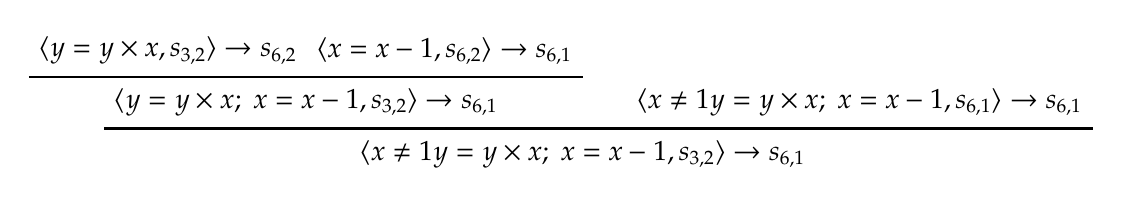
\begin{tikzpicture}
   [edge from parent path={
      ($(\tikzchildnode.west) - (0,0.5\tikzleveldistance)$)
      -- ($(\tikzchildnode.east) - (0,0.5\tikzleveldistance)$)
      ($(\tikzparentnode.west) + (0,0.5\tikzleveldistance)$)
      -- ($(\tikzparentnode.east) + (0,0.5\tikzleveldistance)$)
    },
    grow'=up,
    level/.style={sibling distance=20em/#1},
    level distance=4ex]
    \node {$\<\WHILE x \neq 1 \DO y = y \times x\COMP x = x - 1, s_{3,2}\> \to s_{6,1}$}
    child { node {$\<y = y \times x\COMP x = x - 1, s_{3,2}\> \to s_{6,1}$}
      child { node {$\<y = y \times x, s_{3,2}\> \to s_{6,2}$} }
    child { node {$\<x = x - 1, s_{6,2}\> \to s_{6,1}$} } }
  child { node {$\<\WHILE x \neq 1 \DO y = y \times x\COMP x = x - 1, s_{6,1}\> \to s_{6,1}$} };
\end{tikzpicture}

% vim: ft=context


\backmatter

\end{document}

% vim: ft=context
